\documentclass[10pt,a4paper]{article}
\usepackage[utf8]{inputenc}
\usepackage{listings}
\usepackage[T1]{fontenc}
\usepackage{amsmath}
\usepackage{amssymb}
\usepackage{graphicx}
\usepackage[english]{babel}
\usepackage{listings}
\tracinglostchars=2
\usepackage{iftex}
\pagestyle{empty}
\ifTUTeX
\usepackage{fontspec}
\else
\usepackage[T1]{fontenc}
\usepackage[utf8]{inputenc} % The default since 2018
\DeclareUnicodeCharacter{200B}{{\hskip 0pt}}
\fi

\begin{document}
	\begin{figure*}
		
\includegraphics[scale=0.7]{econpic}
		\centering
	\end{figure*}
	\title { {\Huge Managing Big Data} \\ 
		Second Assignment }
	\author{
		\textbf{Peter Pan} \\
	}
	\date{ 24 / 11 / 2022 }
	
	
	\maketitle
	
	\newpage
	
	\tableofcontents
	
	\newpage
	\section{}
	\section{Subject 2}
Firstly , we use the dataset from the site “UCI Machine Learning Repository ”. This dataset includes facts, that associated with crimes about 10.0000 citizens at U.S.A. (variable ViolentCrimesPerPop) with social and financial details for each area(Communities and Crime Data Set).Then we do the following linear regression at the environment of R:\\
	\\
ViolentCrimesPerPop=b0+b1medIncome+b2whitePerCap
+b3blackPerCap+b4HispPerCap\\+b5NumUnderPov
+b6PctUnemployed+b7HousVacant+b8MedRent+b9NumStreet\\
	
At the file "communities.data" ,we replace the names of the variables with the names of file "communities.names". Then we remove lines that have not avaliable data , and we create a new data set in which we do OLS in order to create coefficients.
	
	\subsection{Task I in R}
	\begin{lstlisting}[language=R]
setwd("C:/Users/user/Desktop/shls")
communities <- read.csv("communities.data", header=FALSE)
	\end{lstlisting}
colnames(communities) <- c("state", "county", "community", "communityname","fold", "population", "householdsize", "racepctblack", "racePctWhite", 
	"racePctAsian", "racePctHisp", "agePct12t21", "agePct12t29", "agePct16t24", "agePct65up", "numbUrban", "pctUrban", "medIncome", "pctWage", "pctWFarmSelf", "pctWInvInc", "pctWSocSec", "pctWPubAsst", "pctWRetire", "medFamInc", "perCapInc","whitePerCap", "blackPerCap", "indianPerCap", "AsianPerCap", "OtherPerCap", "HispPerCap", "NumUnderPov", "PctPopUnderPov", "PctLess9thGrade","PctNotHSGrad", "PctBSorMore", "PctUnemployed", "PctEmploy", "PctEmplManu", "PctEmplProfServ", "PctOccupManu", "PctOccupMgmtProf", "MalePctDivorce","MalePctNevMarr", "FemalePctDiv", "TotalPctDiv", "PersPerFam", "PctFam2Par", "PctKids2Par", "PctYoungKids2Par", "PctTeen2Par", "PctWorkMomYoungKids","PctWorkMom", "NumIlleg", "PctIlleg", "NumImmig", "PctImmigRecent", "PctImmigRec5", "PctImmigRec8", "PctImmigRec10", "PctRecentImmig", "PctRecImmig5","PctRecImmig8", "PctRecImmig10", "PctSpeakEnglOnly", "PctNotSpeakEnglWell", "PctLargHouseFam", "PctLargHouseOccup", "PersPerOccupHous", "PersPerOwnOccHous","PersPerRentOccHous", "PctPersOwnOccup", "PctPersDenseHous", "PctHousLess3BR", "MedNumBR", "HousVacant", "PctHousOccup", "PctHousOwnOcc","PctVacantBoarded", 
	"PctVacMore6Mos", "MedYrHousBuilt", "PctHousNoPhone", "PctWOFullPlumb", "OwnOccLowQuart", "OwnOccMedVal", "OwnOccHiQuart", "RentLowQ", "RentMedian","RentHighQ", "MedRent", "MedRentPctHousInc", "MedOwnCostPctInc", "MedOwnCostPctIncNoMtg","NumInShelters","NumStreet", "PctForeignBorn", "PctBornSameState","PctSameHouse85", "PctSameCity85", "PctSameState85", "LemasSwornFT", "LemasSwFTPerPop", "LemasSwFTFieldOps", "LemasSwFTFieldPerPop", "LemasTotalReq", 
	"LemasTotReqPerPop", "PolicReqPerOffic", "PolicPerPop", "RacialMatchCommPol", "PctPolicWhite", "PctPolicBlack", "PctPolicHisp", "PctPolicAsian", "PctPolicMinor", "OfficAssgnDrugUnits", "NumKindsDrugsSeiz", "PolicAveOTWorked", "LandArea", "PopDens", "PctUsePubTrans", "PolicCars", "PolicOperBudg", 
	"LemasPctPolicOnPatr", "LemasGangUnitDeploy", "LemasPctOfficDrugUn", "PolicBudgPerPop", "ViolentCrimesPerPop")\\
	\begin{lstlisting}	
com.na <- replace(communities, communities=="?", NA)
		
newdata <- na.omit(com.na)
		
linear.regression.model<-
lm(ViolentCrimesPerPop ~ medIncome+whitePerCap
+blackPerCap+HispPerCap+NumUnderPov+
PctUnemployed+HousVacant+MedRent+NumStreet, data=newdata)
		
print( linear.regression.model\$coefficients )
summary(linear.regression.model)
	\end{lstlisting}

	\subsection{Task II in Python}
	import statistics\\
	from numpy import nan\\
	from sklearn import datasets, linea\_model, metrics\\
	
	import pandas as pd\\
	import matplotlib.pyplot as plt\\
	
	communities = pd.read\_csv("communities.data", header=0, sep=",")\\
	communities = communities.set\_axis(["state", "county", "community", "communityname", "fold", "population", "householdsize", "racepctblack", "racePctWhite", "racePctAsian",
	"racePctHisp", "agePct12t21", "agePct12t29", "agePct16t24", "agePct65up", "numbUrban", "pctUrban", "medIncome", "pctWage", "pctWFarmSelf", 
	"pctWInvInc", "pctWSocSec", "pctWPubAsst", "pctWRetire", "medFamInc", "perCapInc",
	"whitePerCap", "blackPerCap", "indianPerCap", "AsianPerCap", "OtherPerCap", "HispPerCap", "NumUnderPov", "PctPopUnderPov", "PctLess9thGrade",
	"PctNotHSGrad", "PctBSorMore", "PctUnemployed", "PctEmploy", "PctEmplManu", "PctEmplProfServ", "PctOccupManu", "PctOccupMgmtProf", "MalePctDivorce",
	"MalePctNevMarr", "FemalePctDiv", "TotalPctDiv", "PersPerFam", "PctFam2Par", "PctKids2Par", "PctYoungKids2Par", "PctTeen2Par", "PctWorkMomYoungKids",
	"PctWorkMom", "NumIlleg", "PctIlleg", "NumImmig", "PctImmigRecent", "PctImmigRec5", "PctImmigRec8", "PctImmigRec10", "PctRecentImmig", "PctRecImmig5",
	"PctRecImmig8", "PctRecImmig10", "PctSpeakEnglOnly", "PctNotSpeakEnglWell", "PctLargHouseFam", "PctLargHouseOccup", "PersPerOccupHous", "PersPerOwnOccHous",
	"PersPerRentOccHous", "PctPersOwnOccup", "PctPersDenseHous", "PctHousLess3BR", "MedNumBR", "HousVacant", "PctHousOccup", "PctHousOwnOcc", "PctVacantBoarded", 
	"PctVacMore6Mos", "MedYrHousBuilt", "PctHousNoPhone", "PctWOFullPlumb", "OwnOccLowQuart", "OwnOccMedVal", "OwnOccHiQuart", "RentLowQ", "RentMedian",
	"RentHighQ", "MedRent", "MedRentPctHousInc", "MedOwnCostPctInc", "MedOwnCostPctIncNoMtg", "NumInShelters", "NumStreet", "PctForeignBorn", "PctBornSameState",
	"PctSameHouse85", "PctSameCity85", "PctSameState85", "LemasSwornFT", "LemasSwFTPerPop", "LemasSwFTFieldOps", "LemasSwFTFieldPerPop", "LemasTotalReq", 
	"LemasTotReqPerPop", "PolicReqPerOffic", "PolicPerPop", "RacialMatchCommPol", "PctPolicWhite", "PctPolicBlack", "PctPolicHisp", "PctPolicAsian", 
	"PctPolicMinor", "OfficAssgnDrugUnits", "NumKindsDrugsSeiz", "PolicAveOTWorked", "LandArea", "PopDens", "PctUsePubTrans", "PolicCars", "PolicOperBudg", 
	"LemasPctPolicOnPatr", "LemasGangUnitDeploy", "LemasPctOfficDrugUn", "PolicBudgPerPop", "ViolentCrimesPerPop"], axis=1)\\
	
	communities\_nan = communities.replace('[?]', np.nan, regex=True)\\
	
	
	communitiesnew=communities\_nan.dropna()\\
	print(communitiesnew)\\
	
	independentVariables = communitiesnew.loc[:, ["medIncome", "whitePerCap","blackPerCap", "HispPerCap", "NumUnderPov", "PctUnemployed", "HousVacant", "MedRent", "NumStreet"]]\\
	
	dependentVariable = communitiesnew.loc[:, "ViolentCrimesPerPop"]\\
	
	reg = linear\_model.LinearRegression()\\
	
	reg.fit(independentVariables, dependentVariable )\\
	
	print('Coefficients: ', reg.coef\_)\\
	print(f"intercept: {reg.intercept\_}")\\
	\\
	\subsection{Task III in Python}
By using the method of Batch Gradient Descent ,at the data set "Communities and Crime Data Set" we make a program that estimates the coefficients of the linear model of the query i\\
The results, we get  are different each time we run the program as randomly takes "$\theta$"\\
	\begin{lstlisting}[language=R]
import numpy as np
import pandas as pd
import matplotlib.pyplot as plt
import warnings
	
warnings.filterwarnings('ignore')
	\end{lstlisting}
	
\# Multiply two matrices i.e. mat1 * mat2
\begin{lstlisting}[language=R]
def matmultiply(mat1,mat2):
	
return( np.matmul(mat1, mat2) )
\end{lstlisting}
\#Calculate current value of cost function J($\theta$).
\#indV: matrix of independent variables, first column must be all 1s\\
\#depV: matrix (dimensions nx1)of dependent variable i.e.\\
\begin{lstlisting}[language=R]	
def calculateCost(indV, depV, thetas):
return( np.sum( ((matmultiply(indV, thetas) - depV)**2) / (2*indV.shape[0]) ) )  
\end{lstlisting}
	

\#Batch gradient descent\\

\#indV:matrix of independent variables, first column must be all 1s\\
\#depV: matrix (dimensions nx1)of dependent variable i.e.\\
\# alpha: value of learning hyperparameter. Default (i.e. if no argument provided)  0.01\\
\# numIters: number of iterations. Default (i.e. if no argument provided) 100\\
\begin{lstlisting}[language=R]	
def batchGradientDescent(indV, depV, thetas, alpha=0.1, numIters=200
, verbose=False):
calcThetas = thetas
costHistory = pd.DataFrame(columns=["iter", "cost"])
m = len(depV)
for i in range(0, numIters):
prediction = np.dot(indV, calcThetas)
calcThetas = calcThetas - (1 / m) * alpha * (indV.T.dot(prediction - depV))
print(">>>> Iteration", i, ")")
print("       Calculate thetas...", calcThetas)
c = calculateCost(indV, depV, calcThetas)
print("       Calculate cost fuction for new thetas...", c)
costHistory = costHistory.append({"iter": i, "cost": c}, ignore_index=True)
return calcThetas, costHistory
	
\end{lstlisting}	
	
communities = pd.read\_csv("communities.data", header=None, sep=",", engine='python')
communities = communities.set\_axis(["state", "county", "community", "communityname", "fold", "population", "householdsize", "racepctblack", "racePctWhite", "racePctAsian",
"racePctHisp", "agePct12t21", "agePct12t29", "agePct16t24", "agePct65up", "numbUrban", "pctUrban", "medIncome", "pctWage", "pctWFarmSelf", 
"pctWInvInc", "pctWSocSec", "pctWPubAsst", "pctWRetire", "medFamInc", "perCapInc",
"whitePerCap", "blackPerCap", "indianPerCap", "AsianPerCap", "OtherPerCap", "HispPerCap", "NumUnderPov", "PctPopUnderPov", "PctLess9thGrade",
"PctNotHSGrad", "PctBSorMore", "PctUnemployed", "PctEmploy", "PctEmplManu", "PctEmplProfServ", "PctOccupManu", "PctOccupMgmtProf", "MalePctDivorce","MalePctNevMarr", "FemalePctDiv", "TotalPctDiv", "PersPerFam", "PctFam2Par", "PctKids2Par", "PctYoungKids2Par", "PctTeen2Par", "PctWorkMomYoungKids",
"PctWorkMom", "NumIlleg", "PctIlleg", "NumImmig", "PctImmigRecent", "PctImmigRec5", "PctImmigRec8", "PctImmigRec10", "PctRecentImmig", "PctRecImmig5",
"PctRecImmig8", "PctRecImmig10", "PctSpeakEnglOnly", "PctNotSpeakEnglWell", "PctLargHouseFam", "PctLargHouseOccup", "PersPerOccupHous", "PersPerOwnOccHous",
"PersPerRentOccHous", "PctPersOwnOccup", "PctPersDenseHous", "PctHousLess3BR", "MedNumBR", "HousVacant", "PctHousOccup", "PctHousOwnOcc", "PctVacantBoarded", 
"PctVacMore6Mos", "MedYrHousBuilt", "PctHousNoPhone", "PctWOFullPlumb", "OwnOccLowQuart", "OwnOccMedVal", "OwnOccHiQuart", "RentLowQ", "RentMedian",
"RentHighQ", "MedRent", "MedRentPctHousInc", "MedOwnCostPctInc", "MedOwnCostPctIncNoMtg", "NumInShelters", "NumStreet", "PctForeignBorn", "PctBornSameState",
"PctSameHouse85", "PctSameCity85", "PctSameState85", "LemasSwornFT", "LemasSwFTPerPop", "LemasSwFTFieldOps", "LemasSwFTFieldPerPop", "LemasTotalReq", 
"LemasTotReqPerPop", "PolicReqPerOffic", "PolicPerPop", "RacialMatchCommPol", "PctPolicWhite", "PctPolicBlack", "PctPolicHisp", "PctPolicAsian", 
"PctPolicMinor", "OfficAssgnDrugUnits", "NumKindsDrugsSeiz", "PolicAveOTWorked", "LandArea", "PopDens", "PctUsePubTrans", "PolicCars", "PolicOperBudg", 
"LemasPctPolicOnPatr", "LemasGangUnitDeploy", "LemasPctOfficDrugUn", "PolicBudgPerPop", "ViolentCrimesPerPop"], axis=1)
\begin{lstlisting}[language=R]	
dependentVar = communities.iloc[:, 127]
\end{lstlisting}
\# These are all our independent ones:\\ 17,26,27,31,32,37,76,90,95\\
\# above indecies are 0-based!\\
\begin{lstlisting}[language=R]	
independentVars = communities.iloc[:, [17,26,27,31,32,37,76,90,95] ]
	
independentVars = independentVars[(independentVars != '?').all(1)]
	
independentVars.insert(0, 'b0', 1)
\end{lstlisting}
\# Initialize thetas with some random values.\\
\# We'll need (independentVars.shape[1])  theta values, one for each independent variable.\\
\begin{lstlisting}[language=R]		
independentVars etc
iniThetas = []
for i in range(0, independentVars.shape[1]):
iniThetas.append( np.random.rand() )
	
initialThetas = np.array(iniThetas)
\end{lstlisting}	
	
\#we run BATCH gradient descent and return 2 values: \\
\begin{lstlisting}[language=R]	
estimatedCoefficients, costHistory =
 batchGradientDescent(independentVars.to_numpy(), dependentVar.to_numpy()
 ,initialThetas, 0.1, 200)
	
	print(estimatedCoefficients)
\end{lstlisting}		
\# Display the cost function to see if alpha and number of iterations were appropriate.
\begin{lstlisting}[language=R]	
costHistory.plot.scatter(x="iter", y="cost", color='red')
plt.show()
\end{lstlisting}	
\#There is the graph of the cost function values ​​as
function of the number of iterations:
\\
\vspace{2cm}
{\scalebox{0.6}{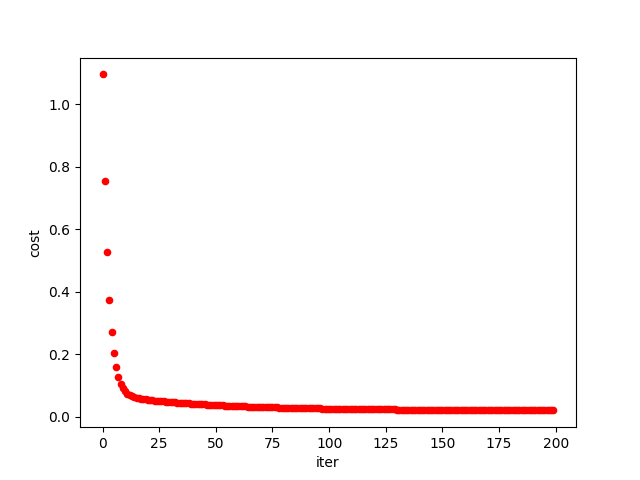
\includegraphics{Figure_1}}}
\\[0.5cm]
\bigskip  \bigskip

	
	\section{Subject 3}
	\subsection{Task I }
The program which is given, is a program in the  environment of R ,that  initially, creates a data frame called 'myData'. It's an empty set with only 7 columns that take numeric values and it isn’t defined the number of rows :
	\begin{lstlisting}[language=R]
myData <- data.frame(y=numeric(0),
x1=numeric(0), 
x2=numeric(0), 
x3=numeric(0), 
x4=numeric(0), 
x5=numeric(0), 
x6=numeric(0))
	\end{lstlisting}
Consequently, the command "for" creates 4 lines and assigns 7 values between 1 and 10 for each variable of the set.Each time we run it, the command will assign different values for each position of my data Frame:
	\begin{lstlisting}[language=R]
for (i in 1:4){
myData[i,] <- runif(7, min=1, max=10)
	}
	\end{lstlisting}
Then the command "rModel" actualizeinear regression between the dependent variable "y" and the independent "x1", "x2", "x3", "x4", "x5", "x6". Conclusively, with command "print" we figure the estimated coefficients of our rmodel model. 
	\begin{lstlisting}[language=R]
rModel<-lm( y ~ ., data=myData)
print(rModel$coefficients)
	\end{lstlisting}
	\subsection{Task II }
The values ​​we get from the program  concern only the constant term and variables "x1", "x2", "x3". This is showned in the fact that OLS regression can't work when the number of observations is greater than the number of variables. In order to meet the criteria that required for the estimation of coefficients b linear pulsetion becomes up to "x3" variable.\\
More specifically,just as a matrix must be square to be inverted and executed, so in our example only the first four factors of b are shown along with the constant term.
	If we had given the command:
	\begin{lstlisting}[language=R]
for (i in 1:7)
	\end{lstlisting}
it could print obsarvations for all x.
Finnaly , we use two examples to make the square of factor b more understandable:
firstly , we create with the command 
	\begin{lstlisting}[language=R]
for (i in 1:7)
	\end{lstlisting}
we create a table with 7 rows and 6 columns.
In the second example  with the command:
	\begin{lstlisting}[language=R]
for (i in 1:5)
	\end{lstlisting}
we create a table with 5 rows and 6 columns.
In this wy,we get estimated values only up to x4 (with the fixed term) 10
	\newpage
	\section{Subject 4}
In this article, we use a dataset of criminal trials in Florida from 2000 to 2010 to examine the impact of juror ethnic composition on trial outcomes. (ii) this gap in conviction rates is completely eliminated if the jury pool includes at least one black member; The trial in Florida has her six jurors. 401 of the 785 felony jury trials are from Sarasota County, and 384 are from Lake County, leaving us with a data set of 785 such trials.
	
We find that jurors of at least one race (and possibly both) either interpret the evidence differently depending on the race of the defendant or apply a standard of evidence that differs depending on the race of the defendant in the 712 trials in which the primary dependent variables are defined and the defendant is identified as either being black (n = 333) or white (n = 379). In order to ensure the fairness of the criminal justice system, the impact of the racial composition of the jury pool (and seated jury) is a factor that merits much more attention and analysis. This is because both possibilities imply that the interaction of defendant and jury race fundamentally alters the mapping of evidence to conviction rates.
	\subsection{Task I}
As the dependent variable we have the result of the linear regression of the independent variables that we use each time. Specifically the dependent variables are :\\
	\begin{itemize}
		\item \emph Any guilty
		\item \emph	Conviction
		\item \emph	Proportion guilty convictions 
		\item \emph	Number of seated
		\item \emph	Number in jury poo
		\item \emph	Any black in Pool
		\item \emph	Any black on Seated jury 
		\item \emph	Proportion black on seated jury
		\item \emph Proportion black in pool 
	\end{itemize}
	The independent variables of the article are:
	\begin{itemize}
		\item \emph	Any drug conviction
		\item \emph	Any violent conviction 
		\item \emph	Any property conviction
		\item \emph Black Defendant 
		\item \emph any black in pool
		\item \emph Defendant black * any black in pool 
		\item \emph Gender large of pool
		\item \emph Country dummy
		\item \emph Years of filing dummies
		\item \emph Any black on seated jury
		\item \emph Defendant black * any black on seated jury
	\end{itemize}		
	
	\subsection{Task II}
The forms of regression models that used in the article are two :
	\begin{itemize}
		\item \emph $y_i = b_0 + b_1X_{1i} + b_2X_{2i} + ... $     
		\item \emph $y_i = b_0 + b_1X_{1i} + b_2X_{2i} + b_3X_{1i}X_{2i} ... $
		\item \emph $y_i = b_0 + b_1X_{1i} + b_2X_{2i} +b_3X_{3i} + b_4X_{1i}X_{2i} + b_5X_{1i}X_{3i} ... $
	\end{itemize} 
in the above regression models, $X_{1i}, X_{2i}$ are the dependent variables and $Y_i$ are the independent variables  
	\subsection{Task III}
The method which is used is the least squares method which is a method of estimating coefficients b of a linear regression model, which is knowned as "OLS" method.\\
	\subsection{Task IV}
The aim of the study is the explanation of the dependent variable since it analyzes data that lead to a conclusion. Study shows racial bias among jurors. More specifically the jurors of at least one race:
	\begin{itemize}
		\item \emph interpret the evidence differently depending on the race of the accused
		\item \emph use a standard of evidence that varies with the race of the defendant
	\end{itemize}
In this way , both The racial composition of the jury and the sitting committee are affected , so the award of justice loses its essential character of justice.
	\newpage
	\section{Subject 5}
	\begin{lstlisting}[language=R]
setwd("D:/EfarmMakro/tzagkarakis")
HouseholdData<-read.csv("HouseholdData.csv", sep=",", header=T)

linear.regression.model<-lm(FoodExpenditure ~ Income + FamilySize, data=HouseholdData)

print( linear.regression.model$coefficients )

summary(linear.regression.model)

calculateCost<-function(X, y, theta){
m <- length(y)
return( sum((X%*%theta- y)^2) / (2*m) )
} 
gradientDescent<-function(X, y, theta, alpha=0.01, numIters=90){
m <- length(y)	
costHistory <- rep(0, numIters)	
for(i in 1:numIters){	
theta <- theta - alpha*(1/m)*(t(X)%*%(X%*%theta - y))	
costHistory[i]  <- calculateCost(X, y, theta)		
} 
gdResults<-list("coefficients"=theta, "costs"=costHistory)
return(gdResults)
} 
numObs<-nrow(HouseholdData)

revenue<- HouseholdData[, 2]

indVariables<- cbind( rep(1, numObs), HouseholdData$Income, HouseholdData$FamilySize ) 

initialThetas<-rep(runif(1), 3) 

gdOutput<-gradientDescent(indVariables, revenue, initialThetas, 0.000000000001, 20000)

print(gdOutput$coefficients)

plot(gdOutput$costs, xlab="number of repetitions", ylab="J(\theta)" )

	
	\end{lstlisting}
	\newpage
	
After we wrote a program in R that estimates the coefficients of the following multiple linear regression model using the Least Squares method and the Stepped Down Beam method, the results we obtained are listed below.
	The results of the least squares method are as follows:\\
	\begin{table}[results of the least squares method]
		\begin{tabular}{1|1|1|1|1}
			&	Estimate Std. & Error t value & PR(>|t|) \\
			Intercept & 1.182e+03 & 8.269e+02 & 1.430  0.1625 \\
			Income & 1.224e-01 & 7.276e-03 & 16.817 <2e-16*** \\
			FamilySize & 3.257e+02 & 1.533e+02 & 2.124 0.0415*\\
		\end{tabular}		
	\end{table}
	\\
The results of the Step Down Beam are as follows:\\
	\begin{table}[results of the Step Down Beam]
		\begin{tabular}{1|1}
			& [,1]\\
			Intercept & 0.5594858 \\
			Income & 0.1641353 \\
			FamilySize & 0.5620243 \\
		\end{tabular}		
	\end{table}
	\subsection{Task I }
Between these methods a difference is observed in the estimates of the coefficients they produce. The observed difference is mainly due to the fact that the Gradual Descent method approaches the coefficients with an iterative process as mentioned and consequently the number of repetitions will have an impact on the final estimates as well as the initialization values of the coefficients. Different number of iterations and different initial coefficient values may result in different estimates.
	\subsection{Task II }
What we observe is that there is a big difference between the coefficients estimated by the 2 different models. This is due to the fact that the Gradient Descent algorithm presents an issue regarding the rate of convergence of the coefficients in each iteration. Due to the large difference between the independent coefficients in terms of their sizes (Income min=20000, max=97000) and (FamilySize min=2, max=5), the respective coefficients will converge at a different rate to their appropriate value, which minimizes the cost function. The speed of convergence of the coefficients in the Gradient Descent method is generally sensitive to the measurement scale of the data. In data with such characteristics, one treatment is to normalize the data, which is done in the preprocessing phase, where the data are transformed so that the values of all independent variables have the same measurement scale and their values are in the same range honorably. Common data normalization methods are the Min-Max method which results in all values of a variable being plotted in the value range [0,1].
	
	
\section{Subject 6}
\subsection{Task I in Python}
In terms of generating code in python we have the following:\\
First, the necessary packages are used with the necessary commands:\\
import pandas as pd\\
import numpy as np\\
import random\\
import matplotlib.pyplot as plt\\
from random import seed\\
from random import randint\\
\\

We define the  Stochastic Gradient Descent cost function:\\
def stochasticGradientDescent(x, y, theta, alpha, m, numIters):\\
create and ampty array to save costs:\\
calculatedCosts = []\\

We choose one random observasion to use in sgd:\\
i = random.randint(0, len(dependent) - 1)\\

Now we start the iteration:\\
for k in range(0, numIters):\\
prediction= 0\\
for j in range(10):\\
prediction = prediction + (x[i, j]* thetas[j])\\

we calculate the new theta:\\
newtheta = thetas[j] - alpha * (x[i, j]* (x[i, j]* thetas[j] - y[i]))
theta[j] = newtheta\\

we calculate the cost:\\
cost = ((prediction - y[i]) ** 2) / (2 * m)\\
calculatedCosts.append(cost)\\
print(f"===== Iteration ({k}) ======")\\
print(theta)\\
print(cost)\\
return theta, calculatedCosts\\

We enter the data into the crime variable:\\
Crime = pd.read\_csv("communities.data", header=None, sep=",", engine='python')\\
print(Crime)\\

We find in column 127 the requested dependent variable ViolentCrimesPerPop and create a vector we call df1 containing the values of column 127. Then we print this vector:\\
df1 = Crime.loc[:, [127]]\\
print(type(df1))\\

We convert the dataframe into a matrix using the numpy package:\\
dependent = df1.to\_numpy()\\
print(type(dependent))\\
random\_obs= randint(0, 1994)\\

All our independent variables are in columns 17,26,27,31,32,37,76,90,95 so we create and print a new vector df2 containing all the independent variables:\\
df2 = Crime.loc[:, [17, 26, 27, 31, 32, 37, 76, 90, 95]]\\
print(type(df2))\\

We also convert and print this dataframe into a matrix using the numpy package:\\
independentVars = df2.to\_numpy()\\
print(type(independentVars))\\

We create another table with dimension 1994 rows and a column where all rows take the value 1:\\
onesColumn = np.ones((1994, 1))\\
independentVars = np.hstack((onesColumn,independentVars))\\

Then we give the value of the learning parameter a and define the number of iterations that affect the final estimates of coefficients $\theta$ that will result from Stochastic gradient Descent and terminate this iterative process:\\
set alpha, theta and number of iterations
alpha = 0.1\\
iniThetas = []\\
for i in range(0, independentVars.shape[1]):\\
iniThetas.append( np.random.rand() )\\
thetas = np.array(iniThetas)\\
numIters = 10000\\

Finally we estimate the final stochastic gradient descent function, we print the estimated $\theta$ and to see if the appropriate values have been given to a and the number of iterations and we diagram the cost function:\\
estimatedThetas, costs = stochasticGradientDescent(independentVars, dependent, thetas, alpha, 1994, numIters)\\
print(">>> Estimated thetas")\\
print(estimatedThetas)\\
plt.title('Cost Function J')\\
plt.xlabel('No. of iterations')\\
plt.ylabel('Cost')\\
plt.plot(list(range(numIters)), costs, '-r')\\
plt.show()\\
\\
\\
\\
\\
\\
\\
\\


\begin{figure*}
	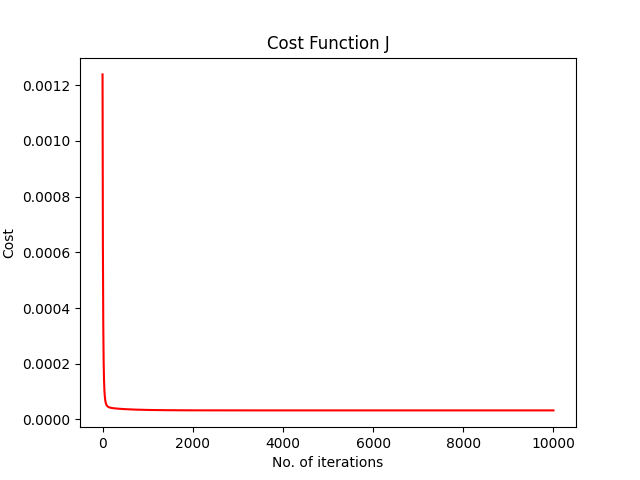
\includegraphics[scale=0.7]{Figure}
	\centering
\end{figure*}


	
\subsection{Task I in R}
	Regarding the creation of the code in R, we have the following results:\\
	First we make use of the libraries to be used, define the place we will work in, import the data set Communities and Crime Data Set, find what type of file the variable communities we have imported is and the number of observations it contains.\\
	library(quantmod)\\
	library(AER)\\
	library(ggplot2)\\
	
	setwd("C:/metaptyxiako/diaxeirhsh megalwn dedomenwn")\\
	communitiesdata <- read.csv("C:/metaptyxiako/diaxeirhsh megalwn dedomenwn/communities.data", header=FALSE,stringsAsFactors = TRUE)\\
	class(communitiesdata)\\
	numObs<- nrow(communitiesdata)\\
	
	We enter in the random sample variable a random sample from the communities data set:\\
	randomobservations <- sample(communitiesdata)\\
	
	We create and calculate the cost function:\\
	ViolentCrimesPerPop <- function(x,y ,theta)\{\\
	\\
	return (sum((x\%*\%theta- y)\^2)/(2*numObs))\\
	\\
	\}\\
	
	We create the gradient descent function, set the learning parameter a=0.01, the number of repetitions of $\theta$ calculation and then calculate the coefficients:\\
	
	gradientDescent<-function(x, y, theta, alpha=0.01, numIters=90)\{\\
	\\
	CrimesHistory <- rep(0, numIters)\\
	\\
	for(k in 1:numIters)\{\\
	\\
	for (i in 1:numObs)\{\\
	\\
	for (j in 1:10)\{\\
	
	newtheta<-theta[j] - alpha * (x[i, j]*(x[i, j] * theta[j] - y[i]))\\
	theta[j]<-newtheta\\
	\}\\
	CrimesHistory[i]  <- ViolentCrimesPerPop(x, y, theta)\\
	\}\\
	\}\\
	gdResults<-list("coefficients"=theta, " ViolentCrimes"= CrimesHistory)\\
	return(gdResults)\\
	\}\\
	
	We put in the variable y the dependent variable in x the independent we find the inverse of the matrix:
	
	y <- communitiesdata\$V128 \\
	x <- cbind(rep(1, numObs),communitiesdata\$V18,communitiesdata\$V27,communitiesdata\$V28,communitiesdata\$V32,communitiesdata\$V33,communitiesdata\$V38,communitiesdata\$V91,communitiesdata\$V77,communitiesdata\$V96)\\
	transX<- t(x)\\                      
	theta <- matrix(runif(n= 10 , min= 1 , max= 1 ), nrow= 10 )\\
	
	We set the learning parameter a=0.01 and the number of iterations to 100:\\
	numIters = 100\\
	alpha  = 0.01\\
	
	Finally we estimate the final stochastic gradient descent function, we print the estimated $\theta$ and to see if the appropriate values have been given to a and the number of iterations and we diagram the cost function:\\
	gdOutput <- gradientDescent(x,y, theta, alpha, numIters)\\
	gdOutput\\
	plot(gdOutput\$ViolentCrimes, ylab="J$(\theta)$", xlab="Iterations")\\
	print(gdOutput\$coefficients)\\
	warnings()\\
	\\
	\\
	\\
	\\
	\\
	\\
	\\
	
	\begin{figure*}
		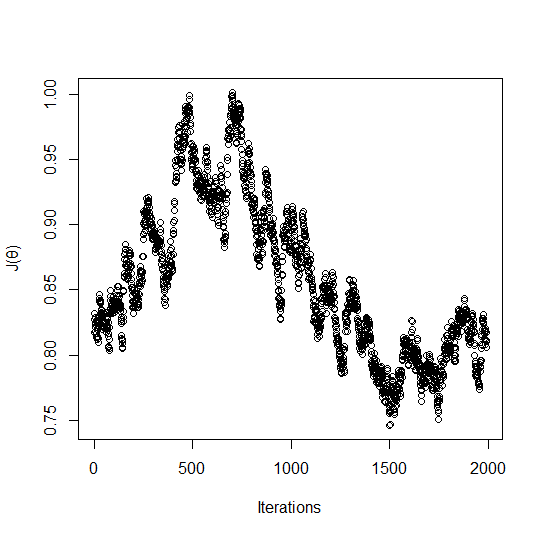
\includegraphics[scale=0.7]{Rplot}
		\centering
	\end{figure*}
	
	
	Regarding the coefficients and for the graph of the cost function values obtained by the Stochastic gradient descent method if we compare them with the coefficients and the cost function values obtained in sub-question ii) of topic 2 where the method was used Batch gradient descent we can conclude in terms of the graphs that the appropriate values of the learning parameter a were used and in both cases, in each iteration of the algorithm the value of the cost function $J(\theta)$ is reduced, the speed with which the reduction is achieved of the cost function is the desired one and this is demonstrated by the final forms of the graphs.Regarding the coefficients of the cost function we notice that in both cases their values have a very small deviation, and each time they differ as the initialization of all the coefficients is done randomly each time when we run the code.
	
	\section{Subject 7}
On this subject we have data about forestfires in Portugal with geografical and meteorogical informations, about the time that a fire broke out, and the area that was burned. Our aim is to predict the area that is going to burned down by estimating the coefficients of the next regrssion model:
	\smallskip
	\[area = b_{1}*temp + b_{2}*wind +b_{3}*rain +b_{0}  \]
	\subsection{Task I in R}
At the beggining we created a function called 'calculateRMSE' to calculate the Root Mean Squared Error.
	\begin{flushleft}
		\begin{lstlisting}[language= R]
calculateRMSE<-function(predictedValues, actualValues){	err<- sqrt(  mean((actualValues - predictedValues)^2))	return( err )}
		\end{lstlisting}
	\end{flushleft}
After that we created a function called 'kFoldCrossValidation' tha will perform the K-Fold Cross validation method on the data set.
	\begin{flushleft}
		\begin{lstlisting}[language=R]
kFoldCrossValidation<-function(data, frml, k){
dataset<-data[sample(nrow(data)),]
folds <- cut(seq(1,nrow(dataset)), breaks=k, labels=FALSE)
RMSE<-vector()
for(i in 1:k){
testIndexes <- which(folds==i,arr.ind=TRUE)
testData <- dataset[testIndexes, ]
trainData <- dataset[-testIndexes, ]
candidate.linear.model<-lm( frml, data = trainData)
predicted<-predict(candidate.linear.model, testData)
error<-calculateRMSE(predicted, testData[, "area"])
MSE<-c(RMSE, error)}
return( mean(RMSE) )}
		\end{lstlisting}
	\end{flushleft}
Then we imported our data from a csv file on a dataframe called forestfires and we tried to omit the NA values but there weren 't any. After that we setted the form of aour prediction model (dependent  and undepent variables).
	\begin{flushleft}
		\begin{lstlisting}[language=R]
forestfires<-read.csv("C:/.../forestfires.csv", sep=",", header=T,
stringsAsFactors = F)
forestfires<-na.omit(forestfires)
predictionModel<-"area ~ temp+wind+rain"
		\end{lstlisting}
	\end{flushleft}
After that we called the 'kFoldCrossValidation' function in our data and we set the argument \( K = 10  \) . In the end we calculate that the prediction error  for our model was 48.577099.
	\begin{flushleft}
		\begin{lstlisting}[language=R]
modelErr<-kFoldCrossValidation(forestfires, as.formula(predictionModel), 10)
modelMeanRMSE<-c(predictionModel, modelErr)
print( sprintf("Linear regression model [%s]: prediction error [%f]",
predictionModel, modelErr ) )
		\end{lstlisting}
	\end{flushleft}\newpage
	\subsection{Task I in Python}
	To begin with we must import the necessary packages.
	\begin{lstlisting}[language=Python]
from sklearn.metrics import mean_squared_error
from sklearn.model_selection import KFold
import numpy as np
import pandas as pd
	\end{lstlisting}
	The next step is to import our data from the csv file and rundomly shuffle it.
	\begin{lstlisting}[language=R]
ffdata = pd.read_csv("C:\\....\\forestfires.csv",
header=0, sep=",", engine='python')
print(ffdata)
ffdata = ffdata.sample(frac=1).reset_index(drop=True)
	\end{lstlisting}
Then we have to use the KFold object from sklearn and set the "K" parameter as ten.After that we will create an array to store the calculated RMSE values and set a counter called "testNumber" equal to zero.
	\begin{lstlisting}[language=Python]
kf = KFold(n_splits=10)
allRMSE = np.empty(shape=[0, 1])
testNumber = 0
	\end{lstlisting}
Next we have to run 'kFoldCrossValidation' on the dataset. On this step we split our dataset on  training data and testing data. We run a linear regresion model on the training data to estimate the coefficients. Then we use the model to predict the value of the dependent variable for the observations in the testing set. After that we calculate the Root Mean Squared Error (RMSE) for this testing set, and we store it on an array.
	\begin{lstlisting}
for train_index, test_index in kf.split(ffdata):
testNumber += 1
trainingData = ffdata.iloc[train_index, :]
testData = ffdata.iloc[test_index, :]
lm = LinearRegression(normalize=False, fit_intercept=True)
estimatedModel = lm.fit(trainingData.loc[:,
['temp', 'wind', 'rain']], trainingData.loc[:, ['area']])
print(">>>Iteration ", testNumber, sep='')
print("\tEstimated coefficients:")
print("\t\tb1=", estimatedModel.coef_[0][0], sep='')
print("\t\tb2=", estimatedModel.coef_[0][1], sep='')		
print("\t\tb3=", estimatedModel.coef_[0][2], sep='')
print("\t\tb0=", estimatedModel.intercept_, sep='')
predictedExpenditure = estimatedModel.predict(testData.loc[:,
['temp', 'wind', 'rain']])
RMSE = sqrt(mean_squared_error(testData.loc[:, ['area']],
predictedExpenditure))
print("\t\tModel RMSE=", RMSE, sep='')
allRMSE = np.append(allRMSE, RMSE)
	\end{lstlisting}
	In the end we calculate the mean RMSE which gives a better estimate on how accurate the predictions of the linear regression model is for unknown data. The mean RMSA is equal to 47.459631. \newpage
	\begin{lstlisting}
print("\n=======================================================")
print(" Final result: Mean RMSE of tests:", statistics.mean(allRMSE), sep='' )
print("=======================================================")
	\end{lstlisting} \newpage
	\subsection{Task II in R}
For Task II we created a subset of the datafream 'forestfires' tha includes the observetions tha the variable 'area'has value les than $3.2$. Then we called again the faction 'kFoldCrossValidation'  for $K = 10$ and we printed the prediction error for our model, which was 0.835316.
	\begin{lstlisting}[language=R]
subfore = subset(forestfires, forestfires$area<3.2 )
modelErr<-kFoldCrossValidation(subfore, as.formula(predictionModel), 10)
modelMeanRMSE<-c(modelMeanRMSE, modelErr)
print( sprintf("Linear regression model [%s]: prediction error [%f]",
predictionModel, modelErr ) ) 
	\end{lstlisting} \newpage
	\subsection{Task II in Python}
In Python we created the subset and run the 'kFoldCrossValidation' with parameter "K" as 10. The prediction error was 0.85483.
	\begin{lstlisting}
allRMSE = np.empty(shape=[0, 1])
testNumber = 0
for train_index, test_index in kf.split(ffdata):
testNumber += 1
trainingData = ffdata.iloc[train_index, :]
testData = ffdata.iloc[test_index, :]
lm = LinearRegression(normalize=False, fit_intercept=True)
estimatedModel = lm.fit(trainingData.loc[:, ['temp', 'wind', 'rain']], trainingData.loc[:, ['area']])
print(">>>Iteration ", testNumber, sep='')
print("\tEstimated coefficients:")
print("\t\tb1=", estimatedModel.coef_[0][0], sep='')
print("\t\tb2=", estimatedModel.coef_[0][1], sep='')
print("\t\tb3=", estimatedModel.coef_[0][2], sep='')
print("\t\tb0=", estimatedModel.intercept_, sep='')
predictedExpenditure = estimatedModel.predict(testData.loc[:, ['temp', 'wind', 'rain']])
RMSE = sqrt(mean_squared_error(testData.loc[:, 
['area']], predictedExpenditure))
print("\t\tModel RMSE=", RMSE, sep='')
allRMSE = np.append(allRMSE, RMSE)
	
print("\n=======================================================")
print(" Final result: Mean RMSE of tests:", 
statistics.mean(allRMSE), sep='' )
print("=======================================================")
		
	\end{lstlisting}.
\section {Subject 8}
\subsection{Task I}
\#generate random x
\begin{lstlisting}[language=R]
x = rnorm(20)
y = 3 + 3*x + 190*x^2 + 250*x^3 +200*x^4 +  rnorm(length(x),0,50)
print(y)
	\end{lstlisting}
\#model fitting
\begin{lstlisting}[language=R]
x = rnorm(20) #generate random x
y = 3 + 3*x + 190*x^2 + 250*x^3 +200*x^4 +  rnorm(length(x),0,50) #create y for model
z = x^2
f = x^3
p = x^4

linearmodel = lm(y~x + z + f + p) #model fitting
summary(linearmodel)


calculateRMSE<-function(predictedValues, actualValues){
	err<- sqrt( mean((actualValues - predictedValues)^2)  )
	return( err )
}

kFoldCrossValidation<-function(data, frml, k){
	dataset<-data[sample(nrow(data)),]
	
	folds <- cut(seq(1,nrow(dataset)), breaks=k, labels=FALSE)
	RMSE<-vector()
	
	for(i in 1:k){
		testIndexes <- which(folds==i,arr.ind=TRUE)
		testData <- dataset[testIndexes, ]
		trainData <- dataset[-testIndexes, ]
		training.linear.model<-lm( frml, data = trainData)
		test.linear.model<-lm( frml, data = trainData)
		k = lm( frml, data = trainData)
		r2 = summary(k)$r.squared 
		predicted<-predict(training.linear.model, trainData)
		trainingdataerror<-calculateRMSE(predicted, trainData[, "y"])
		trainerror<-c(RMSE,trainingdataerror)
		
		predicted<-predict(test.linear.model, testData)
		error<-calculateRMSE(predicted, testData[, "y"])
		RMSE<-c(RMSE, error)
	}
	errorlist = c(mean(RMSE),r2 , trainerror)
	return(errorlist )
}


modelMeanRMSE<-vector()
lamodel = cbind.data.frame(y,x,z,f,p)
predictionModels<-vector()
predictionModels[1]<-"y ~ x + z  + f + p "

for (k in 1:length(predictionModels)){
	modelErr<-kFoldCrossValidation(lamodel, as.formula(predictionModels[k]), 10)
	modelMeanRMSE<-c(modelMeanRMSE, modelErr)
	print( sprintf("Linear regression model [%s]: generalization error [%f]", predictionModels[k], modelErr[1] ) )
	print( sprintf("R spuared for the training data is [%f]", modelErr[2] ) )
	print( sprintf("training error is [%f]", modelErr[3] ) )
}
plot(x,y, xlab = "X (random variable)", ylab = "Y", main = "Graphic representation of Overfitting in our random data" ) #plot for data 
smoothspline = smooth.spline(x,y,df = 20) # line fitting 
lines(smoothspline, col = "green")




\end{lstlisting}
\end{document}